\documentclass[table]{beamer}
% \documentclass[table,handout]{beamer}
% \setbeameroption{show notes}
% \setbeameroption{hide notes}
% \setbeameroption{show only notes}
\usepackage{varwidth}

\newif\ifhide
\newif\ifpost
\newif\ifhideclicker

\hidetrue
% \hideclickertrue
% \posttrue

\newcommand{\whiteout}[1]{\textcolor{white}{#1}}
\newcommand{\whiteoutbox}[1]{\fcolorbox{white}{white}{\parbox{\dimexpr \linewidth-2\fboxsep-2\fboxrule}{\whiteout{#1}}}}
\newcommand{\notebox}[1]{\fcolorbox{blue}{white}{\parbox{\dimexpr \linewidth-2\fboxsep-2\fboxrule}{#1}}}

\ifhide%
    \newcommand{\hmask}[1]{\phantom{\varwidth{\linewidth}#1\endvarwidth}}%
\else%
    \newcommand{\hmask}[1]{#1}%
\fi

\ifhide%
    \newcommand{\hignore}[1]{}%
\else%
    \newcommand{\hignore}[1]{#1}%
\fi

\ifpost%
    \newcommand{\nopost}[1]{}%
\else%
    \newcommand{\nopost}[1]{#1}%
\fi

\ifhide%
    \newcommand{\hidebox}[1]{\phantom{\varwidth{\linewidth}#1\endvarwidth}}%
\else%
    \newcommand{\hidebox}[1]{\fbox{\parbox{\linewidth}{#1}}}%
\fi

\ifhide%
    \newcommand{\wbox}[1]{\whiteoutbox{#1}}%
\else%
    \newcommand{\wbox}[1]{\notebox{#1}}%
\fi

% \ifhide%
%     \newcommand{\clickeranswer}[1]{#1}%
% \else%
%     \newcommand{\clickeranswer}[1]{\textbf{\textcolor{blue}{#1}}}%
% \fi

\ifhideclicker%
    \newcommand{\clickeranswer}[1]{#1}%
\else%
    \ifhide%
        \newcommand{\clickeranswer}[1]{#1}%
    \else%
        \newcommand{\clickeranswer}[1]{\textbf{\textcolor{blue}{#1}}}%
    \fi
\fi

\input{../utils/slide-preamble2.tex}
\newcommand{\highlight}[1]{\textcolor{violet}{\textit{\textbf{#1}}}}
\newcommand{\super}[1]{\ensuremath{^{\textrm{#1}}}}
\newcommand{\sub}[1]{\ensuremath{_{\textrm{#1}}}}
\newcommand{\dC}{\ensuremath{^\circ{\textrm{C}}}}
\newcommand{\tb}{\hspace{2em}}
\providecommand{\e}[1]{\ensuremath{\times 10^{#1}}}
\newcommand{\myHangIndent}{\hangindent=5mm}

\makeatletter
\newcommand*{\rom}[1]{\expandafter\@slowromancap\romannumeral #1@}
\makeatother

\newcommand{\blankslide}{{\setbeamercolor{background canvas}{bg=black}
\setbeamercolor{whitetext}{fg=white}
\begin{frame}<handout:0>[plain]
\end{frame}}}

\newcommand{\whiteslide}{
\begin{frame}<handout:0>[plain]
\end{frame}}

\newcommand{\f}[1]{\ensuremath{F_{#1}}}

\bibliography{../bib/references}
\input{../utils/title-info.tex}

\title[Mutualism]{Mutualism}
% \date{\today}
\date{May 26, 2015}

% \setbeamertemplate{section in toc}[sections numbered]
% \setbeamertemplate{subsection in toc}[subsections numbered]

\begin{document}

\begin{noheadline}
\maketitle
\end{noheadline}

\nopost{
\begin{noheadline}
\begin{frame}[c]
    \vspace{-6mm}
    \begin{center} 
        \includegraphics[height=1.2\textheight]{../images/seating-chart-2.pdf}
    \end{center}
\end{frame}
\end{noheadline}
}

\clickerslide{
\begin{noheadline}
\begin{frame}
    \begin{clickerquestion}
        \item Tobacco plants produce nicotine as a defense against
            caterpillars. On average, individuals that are induced to produce
            more nicotine make fewer seeds than non-induced individuals. Why is
            there a cost of defense from consumers---meaning, a fitness
            trade-off?
 
        \begin{clickeroptions}
            \item \clickeranswer{Resources committed to defense can't be used
                    for growth or reproduction.}
            \item It is difficult to produce both standing and induced
                defenses.
            \item Hosts and consumers have coevolved.
            \item Induced defenses are more efficient than standing defenses
                energetically, but take time to produce.
        \end{clickeroptions}
    \end{clickerquestion}
\end{frame}
\end{noheadline}
}

% \clickerslide{
% \begin{noheadline}
% \begin{frame}
%     \begin{clickerquestion}
%         \item According to the tobacco data you reviewed, there did NOT appear
%             to be a cost of nicotine defense in tobacco plants that had
%             experienced intense selection by herbivores. How could this be? 
%  
%         \begin{clickeroptions}
%             \item It is difficult to produce standing AND induced defenses.
%             \item Hosts and consumers have coevolved.
%             \item Induced defenses are more efficient than standing defenses
%                 energetically, but take time to produce.
%             \item \clickeranswer{Due to constant herbivory the tobacco
%                     population evolved to use nicotine as a standing defense.}
%             \item Resources committed to defense can't be used for growth or
%                 reproduction.
%         \end{clickeroptions}
%     \end{clickerquestion}
% \end{frame}
% \end{noheadline}
% }


\begin{noheadline}
\begin{frame}
\frametitle{Today's issues:}
\vspace{5mm}
% \tableofcontents[subsectionstyle=hide]
\tableofcontents
\end{frame}
\end{noheadline}

\section{Treehoppers and ants}

\begin{frame}[t]
    \begin{adjustwidth}{-2em}{-1.5em}
        Recall the treehopper-ant interaction data from the reading

        \begin{itemize}
            \item Why is this interaction ``contingent?''

            \nbox{This mutualistic interaction is contingent upon the density
                of spiders. If there are many spiders around, the fitness of
                both the ants and the hoppers increase. But, if spiders are
                scarce, the interaction becomes parasitic; the ants are
                benefiting from the honeydew, but the hoppers are not gaining
                the benefit of protection to offset the fitness cost of
                producing the honeydew.}
        \end{itemize}
    \end{adjustwidth}
\end{frame}

\clickerslide{
\begin{frame}
    \begin{clickerquestion}
        \item Consider the treehopper-ant interaction data (from the reading).
            Long-term, how would the nature of the interaction change if spider
            density remained low for many generations and ``honeydew''
            production is expensive?
        \begin{clickeroptions}
            \item \clickeranswer{Selection should favor treehoppers that don't
                    release honeydew.}
            \item Selection should favor ants that eat treehoppers.
            \item Selection should favor treehoppers that eat ants.
            \item Ant populations increase (no energy spent defending against
                spiders).
        \end{clickeroptions}
    \end{clickerquestion}

\end{frame}
}

\section{Mycorrhizae and plants}

\begin{frame}[t]
    \begin{adjustwidth}{-2em}{-1.5em}
        \begin{columns}

            \column{0.5\linewidth}

            Mycorrhizal fungi

            \vspace{4mm}
            Fungi growing on roots of plants

            \vspace{4mm}
            What do you notice about this photograph? (tree seedling roots are
            highlighted in red)

            \nbox{LOTS of fungi; much more fungi surface area than plant roots.
                Also, fungi are connecting the roots of different seedlings.}

            \column{0.49\linewidth}

            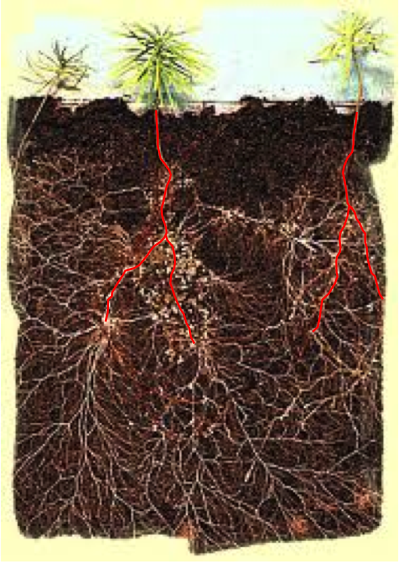
\includegraphics[width=\columnwidth]{roots.png}

        \end{columns}
    \end{adjustwidth}
\end{frame}

% \begin{frame}[t]
%     \begin{adjustwidth}{-2em}{-1.5em}
%         \begin{itemize}[<+->]
%             \item Mushroom-forming fungi are the only organisms
%                 (besides a few bacterial species) that can digest
%                 the lignin found in wood.

%             \item In general, fungi are extremely efficient at
%                 digesting large, complex organic compounds into
%                 small molecules or atoms.

%             \item The body of a fungus has an extremely high surface area for
%                 absorbing water and nutrients.

%         \end{itemize}

%     \end{adjustwidth}
% \end{frame}

\clickerslide{
\begin{frame}
    \begin{clickerquestion}
        \item Describe the nature of the plant-mycorrhizal fungus mutualism.
    \end{clickerquestion}

    \begin{adjustwidth}{-2em}{-1.5em}
    \begin{table}%[htbp]
        \centering
        \begin{tabular}{ l | L{5.2cm} | L{5.2cm} | }
            \multicolumn{1}{c}{} &
            \multicolumn{1}{c}{Plant benefit} &
            \multicolumn{1}{c}{Fungal benefit} \\
            \cline{2-3}
            \textcolor{red}{1)} &
            Protection for roots &
            N and P \\
            \cline{2-3}
            \textcolor{red}{2)} &
            \clickeranswer{N, P, and water} & 
            \clickeranswer{Photosynthate} \\
            \cline{2-3}
            \textcolor{red}{3)} &
            Share nutrients with nearby individuals &
            Connect nearby plants \\
            \cline{2-3}
            \textcolor{red}{4)} &
            Defensive compounds &
            Defensive compounds \\
            \cline{2-3}
        \end{tabular}
    \end{table}
    \end{adjustwidth}
\end{frame}
}

\begin{noheadline}
\begin{frame}[t]
    \begin{adjustwidth}{-2em}{-1.5em}
        \vspace{-7mm}
        \begin{columns}[t]

            \column{0.65\linewidth}

            Experiment:

            \begin{itemize}[<+->]
                \item Grow plant seedlings on culture dishes in the
                    lab, with fungi.

                \item TOP: Add labeled sugar to the plant (top), and zero
                    (left) or lots (right) of phosphate to the fungi.

                \item BOTTOM: Add labeled P to the fungus (top), and zero
                    (left) or lots (right) of sugar to the plant.
            \end{itemize}

            \column{0.34\linewidth}

            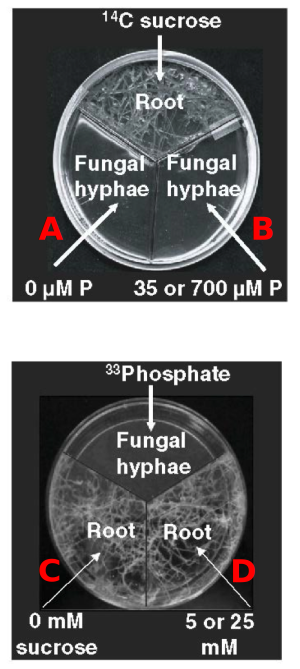
\includegraphics[width=\columnwidth]{fungus-plates.png}

        \end{columns}
    \end{adjustwidth}
\end{frame}
\end{noheadline}

\clickerslide{
\begin{noheadline}
\begin{frame}[t]
    \begin{adjustwidth}{-2em}{-1.5em}
        \vspace{-7mm}
        \begin{columns}[t]

            \column{0.65\linewidth}

            Experiment:

            \begin{itemize}
                \item Grow plant seedlings on culture dishes in the
                    lab, with fungi.

                \item TOP: Add labeled sugar to the plant (top), and zero
                    (left) or lots (right) of phosphate to the fungi.

                \item BOTTOM: Add labeled P to the fungus (top), and zero
                    (left) or lots (right) of sugar to the plant.
            \end{itemize}

            \begin{clickerquestion}
                \item Who gets C (top) and P (bottom)?
            \end{clickerquestion}

            \begin{table}%[htbp]
                \centering
                \begin{tabular}{ l  c  c  }
                    \multicolumn{1}{c}{} &
                    \multicolumn{1}{c}{C (top)} &
                    \multicolumn{1}{c}{P (bottom)} \\
                    \cline{2-3}
                    \textcolor{red}{1)} & A & C \\
                    \textcolor{red}{2)} & A & D \\
                    \textcolor{red}{3)} & B & C \\
                    \textcolor{red}{4)} & \clickeranswer{B} & \clickeranswer{D} \\
                \end{tabular}
            \end{table}

            \column{0.34\linewidth}

            \includegraphics[width=\columnwidth]{fungus-plates-labeled.png}

        \end{columns}
    \end{adjustwidth}
\end{frame}
\end{noheadline}
}

\clickerslide{
\begin{frame}
    \begin{clickerquestion}
        \item Droughts are increasing in many regions due to global warming.
            What is likely to happen to plant-mycorrhizal interactions in these
            regions?
        \begin{clickeroptions}
            \item Plants will drop their relationship with mycorrhizae.
            \item The relationship between plants and mycorrhizae will get
                stronger (more beneficial for both parties).
            \item Mycorrhizae will become parasitic on plants.
            \item \clickeranswer{Plants will become parasitic on mychorrhizae.}
        \end{clickeroptions}
    \end{clickerquestion}
    \nbox{\scriptsize In drought, plants are very dependent on getting water
        from mycorrhizae. Providing water is getting more demanding on
        mychorrhizae, and plants can't provide more sugar to compensate. There
        will be strong selective pressure for plants to ``cheat.''}
\end{frame}
}

\clickerslide{
\begin{frame}
    \begin{clickerquestion}
        \item Human activity is increasing the amount of nitrogen in ecosystems.
            What is likely to happen to plant-mycorrhizal interactions?
        \begin{clickeroptions}
            \item \clickeranswer{Plants will end their relationship with
                    mycorrhizae.}
            \item The relationship between plants and mycorrhizae will get
                stronger (more beneficial for both parties).
            \item Mycorrhizae will become parasitic on plants.
            \item Plants will become parasitic on mychorrhizae.
        \end{clickeroptions}
    \end{clickerquestion}
    \nbox{Plants are often limited by N. If there is plenty around in usable
        form, they do not need the mycorrhizae.}
\end{frame}
}

\section{Nitrogen-fixing bacteria}

\begin{frame}[t]
    \begin{adjustwidth}{-2em}{-1.5em}
        Nitrogen-fixing bacteria

        \begin{itemize}[<+->]
            \item Species of \spp{Rhizobium} and \spp{Frankia} (bacteria)
                colonize root cells in legume-family (and others) plants

            \item The bacterial cells convert molecular nitrogen (N\sub{2}) to
                ammonium (NH$_4^{+}$), which can be further converted and used
                to build proteins and nucleic acids.

            \item Nitrogen-fixation is extremely energy intensive (energy in
                the form of sugars is furnished by the host plant).

        \end{itemize}

    \end{adjustwidth}
\end{frame}

\clickerslide{
\begin{frame}
    \begin{clickerquestion}
        \item The interaction between N-fixing bacteria and host plants is
            extremely specific. A series of complex events occur, each
            requiring certain signaling molecules. From the plant's point of
            view, why? 

        \begin{clickeroptions}
            \item \clickeranswer{Parasitic species could mimic the mutualistic
                    species, and gain entry.}
            \item A great deal of coevolution has occurred.
            \item \clickeranswer{The interaction is limited by fitness
                    trade-offs.}
            \item The association occurs even if nitrogen is abundant in the
                soil.
        \end{clickeroptions}
    \end{clickerquestion}
\end{frame}
}

\clickerslide{
\begin{frame}
    \begin{clickerquestion}
        \item In lab this week you'll be working with plants that associate
            with N-fixing bacteria. Sometimes we find nodules (bacterial
            colonies) and sometimes we don't, even though the bacteria have
            been added. What is the most likely hypothesis for why nodules may
            be missing? 

        \begin{clickeroptions}
            \item \clickeranswer{The plants have enough N.}
            \item The plants are starving for N.
            \item Not enough bacteria have been added.
            \item Not enough individuals of the host plant species are present.
        \end{clickeroptions}
    \end{clickerquestion}
\end{frame}
}

\section{Ants that farm fungi}

\begin{frame}[t]
    \begin{adjustwidth}{-2em}{-1.5em}
        \vspace{-4mm}
        \begin{columns}

            \column{0.65\linewidth}

            Ants and fungi

            \begin{itemize}[<+->]
                \item Leaf-cutting ants farm \spp{Leucoagaricus}
                    fungi in underground colonies and eat them.

                \item A fungus called \spp{Escovopsis} feeds on
                    \spp{Leucoagaricus}

                \item The ants carry bacteria from the genus
                    \spp{Streptomyces} on their bodies. The
                    bacteria produce compounds that are toxic
                    to \spp{Escovopsis}

                \item Leaf-cutter ant colonies also contain bacteria from the
                    genus \spp{Klebsiella}. These bacteria live in the fungal
                    gardens and fix atmospheric N\sub{2} into forms that are
                    used by the \spp{Leucoagaricus} and the ants.
            \end{itemize}

            \column{0.35\linewidth}

            \begin{center}
            \includegraphics[height=0.31\textheight]{ants-1.png}

            \includegraphics[height=0.31\textheight]{ants-2.png}

            \includegraphics[height=0.30\textheight]{ants-3.png}
            \end{center}

        \end{columns}

    \barefootnote{\tiny\shortfullcite{Mueller2002}}
    \end{adjustwidth}
\end{frame}

\begin{frame}[t]
    \begin{adjustwidth}{-2em}{-1.5em}
        Draw and label the associations between \spp{Leucoagaricus} (farmed
        fungus), \spp{Escovopsis} (pathogenic fungus), \spp{Streptomyces}
        (anti-fungal bacterium), \spp{Klebsiella} (N-fixing bacterium), and the
        ants.

        \nbox{Ants eat \spp{Leucoagaricus}}
        \nbox{\spp{Escovopsis} eats \spp{Leucoagaricus}}
        \nbox{\spp{Streptomyces} lives on ants and kills \spp{Escovopsis}}
        \nbox{\spp{Klebsiella} fertilizes \spp{Leucoagaricus}}
    \end{adjustwidth}
\end{frame}

\section{Pollination}
\begin{frame}[t]
    \begin{adjustwidth}{-2em}{-1.5em}
        Pollination

        \begin{itemize}
            \item What is the basis of this mutualism?

                \nbox{Pollinators get nutrients (nectar and pollen); plants
                    get gametes transferred}
        \end{itemize}

    \end{adjustwidth}
\end{frame}

\clickerslide{
\begin{frame}
    \begin{clickerquestion}
        \item Many species of orchids have evolved various forms of deceptive
            pollination by insects. E.g., the flowers mimic a mate or an enemy
            to ``trick'' the insect into trying to mate or fight with the
            flower. What interaction best characterizes deceptive pollination
            evolved?

        \begin{clickeroptions}
            \item \clickeranswer{Parasitism}
            \item Commensalism
            \item Competition
            \item Mutualism
        \end{clickeroptions}
    \end{clickerquestion}

    \barefootnote{\shortfullcite{Jersakova2006}}
\end{frame}
}

\clickerslide{
\begin{frame}
    \begin{clickerquestion}
        \item Under what conditions do you think deceptive pollination
            is most likely to evolve?

        \begin{clickeroptions}
            \item \clickeranswer{The plant population is very limited for
                    resources.}
            \item The insect population is very limited for resources.
            \item The insect population density is very low.
            \item The plant population density is very low.
        \end{clickeroptions}
    \end{clickerquestion}

\end{frame}
}

\end{document}

\clickerslide{
\begin{frame}
    \begin{clickerquestion}
        \item 
        \begin{clickeroptions}
            \item 
            \item 
            \item 
            \item 
        \end{clickeroptions}
    \end{clickerquestion}
\end{frame}
}

\clickerpost{
{
\usebackgroundtemplate{\includegraphics[page=17,width=\paperwidth]{./24-Radiation-extinction.pdf}}
\begin{frame}[t,plain]
    \begin{adjustwidth}{-2em}{-1.5em}
        \cmask{Answer: 3}
    \end{adjustwidth}
\end{frame}
}
}

